\chapter{Introduction}
\label{chp:introduction}
Since the introduction of the Internet on 60's and world wide web (WWW) on 90's, more and more people are connected to each other. Recent research shows that peer-to-peer (P2P) Internet already back at its prime by dominating the traffic as shown in Figure \ref{fig:usage} \cite{2015:internettraffic:sandvine}. User interaction in the Internet community can be expressed in various fashion. Many applications and protocols run on top of P2P system, for instance online gaming, computing, and file sharing. Specifically in file-sharing P2P application, to ensure all users has a flawless experience, it is necessary to make all peers participate. In spite of that, not all the peers consistently share the file. This phenomenon is called \textit{freeriding}.

\begin{figure}[h]
	\centering
	\begin{subfigure}[b]{0.8\textwidth}
		\includegraphics[width=\linewidth]{pics/sandvineeu2015}
		\caption{Sandvine data for 2015 internet usage in Europe}
		\label{fig:usage1}
	\end{subfigure}\\
	\begin{subfigure}[b]{0.8\textwidth}
		\includegraphics[width=\linewidth]{pics/sandvineasia2015}
		\caption{Sandvine data for 2015 internet usage in Asia Pasific}
		\label{fig:usage2}
	\end{subfigure}%
	\caption{Traffic of the Internet by Sandvine \cite{2015:internettraffic:sandvine}}.
	\label{fig:usage}
\end{figure}

\section{The freeriding phenomenon}
Among all the peer-to-peer usage in the Internet, file-sharing is the most popular one. Gnutella was one of the most popular application back in 2000-2007. However, it already shut down because of legal and performance issues. In Gnutella, the majority of users (70\%) stopped to share their files. Moreover, about half of the requests only served by top 1\% of the community \cite{2000:freeridegnutella:adar}. Gnutella suffers from a social phenomenon called \textit{freeriding} on the majority of its users.

Freerider is defined as the user behavior that selfishly consumes all the resource without giving back. It may add vulnerabilities in the system \cite{2000:freeridegnutella:adar}. With only a few of the user provide the service for many, it eventually becomes more centralized than a decentralized system. It also may degrade the system performance \cite{2000:freeridegnutella:adar}. \citeauthor{2000:freeridegnutella:adar} showed that lots of P2P peers are always shown self-interest and rationality that can be considered as freeriding. If freeriders become the majority in file-sharing peer-to-peer system, as they occupy a significant amount of resource, eventually bottleneck in the system will occur. As the time goes, an honest, important peer may not feel satisfied and decided to leave the system bringing crucial files with them. The system then becomes degraded, and sooner or later will be completely left by its peers.

Freeriding can lead to a systematically worse problem called ``tragedy of the commons'' \cite{1968:tragedycommon:hardin}. This problem was popularized by \citet*{1968:tragedycommon:hardin} in \citeyear{1968:tragedycommon:hardin}. This social dilemma emerges because of the overuse and overexploitation in the shared resource without feedback from the user. As \citeauthor{1968:tragedycommon:hardin} stated in his paper: ``Freedom in a commons brings ruin to all'', the uncontrollable participants could selfishly take common, limited resource to fulfill their gain.
% how can egoist cooperate :  The Emergence of Cooperation among Egoists (Robert Axelrod). Solved by tit-for-tat -> good performance. managing supply and demand meulpowder p.7

% freerider behaviour, tit-for-tat result
\textit{Extreme freeriding} is a behavior where one does not upload anything while keep downloading data. In current standards, it rarely happens. Instead, it is more common to find \textit{hit and run} behavior \cite{2011:managesupplydemand:meulpolder}. Hit and run (HnR) is a situation where a user has finished downloading then immediately stop his contribution \cite{2014:sustainabilitytorrent:chen}. Hit and run also often referred as one of the freeriding behavior that peer-to-peer communities wanted to prevent. 

%Despite of that, hit and run often not directly affects end-user. A recent study stated that freerider in \bt~may not degrade performance as long as the swarm has at least one dedicated and available seeders \cite{2015:freeriderinbtcommunity:das}. 

%. One thing that need to take into consideration is that in their research, they only take four communities as dataset 

\section{BitTorrent protocol}
%\todo{terlalu ribet section ini, better to have a diagram of bittorent dan legend, trus jelasin sedikit aja komponnennya ngapain}
%It survives until now because \bt~ is a \textit{protocol} that can be implemented by anyone, instead of service that Napster, Kazaa, and Gnutella used to have. To build a system on top of \bt~environment, it is essential to know the complete view how \bt~work. 
\bt~\cite{2003:bittorrent:cohen}, nowadays, stand as \textit{de facto} file-sharing protocol on top of peer-to-peer network. The \bt~protocol can be implemented by anyone, so it is not limited to any particular service like Gnutella.

% tit-for-tat, choking, unchoke, optimistic unchoke
In general view, \bt~consists of peers who participated in file-sharing and \textit{tracker}. \textit{Tracker} is responsible for monitoring the current files distribution and peers' state in the swarm. \textit{Swarm} is a set of peers formed with the same purpose of downloading or uploading certain files represented in \texttt{.torrent} metadata file. Static \texttt{.torrent} file, which contains information such as tracker addresses and unique hash value of the swarm it represents, is created by a peer who wants to publish their files. Files in a swarm consist of several \textit{pieces} or file chunks. A piece is exchanged by the peers in a particular period. \textit{Seeder} is a type of peer who has complete files and uploads (seed) its pieces to other peers. Leecher is a type of peer who downloads from a particular swarm.

%\textit{Tit-for-tat} in \bt~ encourage users to only upload files to one who also has uploaded his file somewhere else. 
%The \textit{tit-for-tat} ranked peer by its upload amount and speed. Therefore, freeriders always get low priority in this mechanism. In this way, \textit{tit-for-tat} incentivizes for user to upload a file.

% how bittorrent handle freeriding (short term)
\bt~uses \textit{tit-for-tat} mechanism as both reward and punishment method for its peers behavior. This mechanism intended to solve fairness issue introduced by freeriders \cite{2003:bittorrent:cohen}. \textit{Tit-for-tat} mechanism always prioritizes peer who has uploaded something. \textit{Tit-for-tat} valid only in a scope of single torrent. That means the state from one swarm can not be carried to another swarm. This reason causes \textit{tit-for-tat} works best only in short term transaction and limited parties. Nevertheless, \citeauthor{2005:bittorrentcooperation:andrade} showed that \bt~is indeed increased cooperation with only less than 6\% peers have not uploaded anything (extremely freeriding) \cite{2005:bittorrentcooperation:andrade}. As for downloading, \bt~always picks \textit{rarest-first} piece based its availability in the swarm. This technique makes sure that a complete file is distributed in the swarm.

In order to find rarest pieces, piece information on peers is necessary. In \bt, there are four methods to discover and update peer information. Those are using centralized trackers, distributed hash table (DHT), peer exchange (PEX), and local service discovery (LSD). Towards a ``trackerless'' \bt~system, DHT allows each peer to become a tracker. LSD is specialized to find peers in a local network. PEX is a mechanism to efficiently contact a peer directly to exchange up-to-date information.

There are many \bt~\textit{communities} that served as a portal to store \texttt{.torrent} file. In general, a community in \bt~ can be divided into two categories: \textit{public} and \textit{private}. Public community means everybody can join the swarm served by a tracker in that community. In the other hand, private communities are closed community which can be accessed by passing particular requirement \cite{2010:pubpriv:meulpolder, 2014:sustainabilitytorrent:chen}. Typically, private communities have higher performance compared to private communities \cite{2010:pubpriv:meulpolder}. \citeauthor{2010:pubpriv:meulpolder} measured that they have 3-5 times faster download speed compared to public communities \cite{2010:pubpriv:meulpolder}. \textit{Private communities} typically have higher seeder-to-leecher ratio (SLR) that affecting the download speed \cite{2005:bittorrentcooperation:andrade}. In such a community, the administrator may enforce a policy such as \textit{Share Ratio Enforcement} (SRE). SRE define the amount a user need to upload before able to download from the community \cite{2012:economicbt:kash}. 
Higher performance comes with a drawback: in private communities, it is also very difficult to get a new membership and very easy to be kicked out \cite{2013:survivepriv:jia}.

\subsection{Tribler}
\label{section:tribler}
%\todo{taruh diagram lagi supaya enak dibaca, komponen kaya end-to-end encrption, dispersy, jadiin kotak aja trus tulis di legend}
Tribler\footnote{\url{https://www.tribler.org/}} is peer-to-peer file sharing application developed at the Delft University of Technology that compatible with \bt~protocol \cite{2008:tribler:pouwelse}. Tribler is a fully decentralized system focused on security and anonymity. Starts with ABC (Another \bt~Client), Tribler currently provides content discovery, channels concept, and reputation management in fully distributed manner. Tribler was downloaded from the official repository on the latest stable release (6.5.2) as much as 172716 times\footnote{\url{http://www.somsubhra.com/github-release-stats/ ?username=tribler&repository=tribler} (Accessed 7 February 2017)}.

All of the Tribler main components such as end-to-end encryption, channel discovery, and many others relied upon the database and dissemination system called \texttt{Dispersy} \cite{2013:dispersy:zeilemaker}. Dispersy maintains and performs the communication between Tribler peers in fully decentralized manner. Dispersy can circulate the message in one-to-one or one-to-many within a group of node called \textit{community}. Important \textit{communities} are summarized in Table \ref{tbl:community} \cite{2016:tribler-techdebt:vos}. We would like to focus on \textit{channel} community which is a community to distribute swarm among Tribler user. Every user can create his own \textit{channel}, add and remove torrent to it, and maintain its activity. 

%Users can adapt and implement its desired \textit{community} by itself. It is including how, what, and where the communication will occur.

\begin{table}[tbp]
	\centering
	\caption{Overview of implemented Dispersy community in Tribler \cite{2016:tribler-techdebt:vos}.}
	\label{tbl:community}
	\begin{tabular}{|c|p{11cm}|}
		\hline
		\rowcolor[HTML]{EFEFEF} 
		\multicolumn{1}{|c|}{\cellcolor[HTML]{EFEFEF}{\color[HTML]{333333} \textbf{Community Name}}} & \multicolumn{1}{c|}{\cellcolor[HTML]{EFEFEF}{\color[HTML]{333333} \textbf{Purpose}}}                                                                                                                                     \\ \hline
		\textit{AllChannel}                                                                          & Used to discover new channels and to perform remote channel search operations.                                                                                                                                           \\ \hline
		\textit{BarterCast4}\cite{2009:bartercast:meulpolder}                                                                         & While currently disabled, this community was used to spread statistics about the upload and download rates of peers inside the network and has originally been created as a mechanism to prevent free-riding in Tribler. \\ \hline
		\textit{Channel}                                                                             & This community represents a single channel and is responsible for managing torrents and playlists inside that channel.                                                                                                   \\ \hline
		\textit{Multichain}          \cite{2015:multichain:norberhuis}                                                                & This community utilizes the blockchain technology and can be regarded as the accounting mechanism that keeps track of shared and used bandwidth.                                                                         \\ \hline
		\textit{Search}                                                                              & This community contains functionalities to perform remote keyword searches for torrents and torrent collecting operations.                                                                                               \\ \hline
		\textit{(Hidden)Tunnel}                                                                      & This community contains the implementation of the Tor-like protocol that enables anonymity when downloading content and contains the foundations of the hidden seeder services protocol, used for anonymous seeding.     \\ \hline
	\end{tabular}
\end{table}

%Tribler implements several Dispersy \textit{communities} on its core function. \citeauthor{2016:tribler-techdebt:vos} summarize the communities in Tribler. Important features such as channel discovery, search within communities, end-to-end Tor-like operations, and currency mechanism are shown in table \ref{tbl:community}. \textit{Channel} is a collection of torrent that has extra capabilities such as vote system, spam prevention, and comment (social) attributes. 

\section{Rewarding user contribution}
\label{sec:userreward}

\bt~is not enough to tackle HnR behavior. Usually, it is necessary to introduce another layer of rewarding scheme, called \textit{incentive mechanism}. Incentive mechanism is a method to reward the user for its contribution. In some cases, it also fines user for its misconduct. SRE in private community is a good example which increases user contribution and swarm performance. It proves that freeriding behavior can be prevented by proper incentive mechanism. By showing goodness, specifically, by uploading data to others, users should get a reward. However, users are typically selfish and always try to maximize their benefit \cite{2015:incentivep2pgame:kang}.

Incentive mechanism is essential as it is one of the property to increase general performance. \citeauthor{2011:managesupplydemand:meulpolder} discussed several kinds of incentive mechanism that can be combined and complement each other. Those are : (i) direct reciprocity, (ii) indirect reciprocity, (iii) centralized reputation, (iv) decentralized reputation, and (v) currency \cite{2011:managesupplydemand:meulpolder}. \textit{Reciprocity} focused on the relationship between peers. As shown in \ref{fig:reciprocation}, it categorized into two : \textit{downstream} and \textit{upstream}. \textit{Reputation} mechanism is more straightforward. The information of user behavior in the past is stored (centralized or decentralized). This information is iteratively updated and spread through all the peers. Last mechanism is \textit{currency} which uses \textit{credit} to incentivize user. By theory, it can emulate other incentive mechanism by quantifying reputation/help. Because of its wide applicability, we will focus on improving the \textit{currency} mechanism.  \textit{Private communities} with SRE is the most common implementation of currency mechanism. 

\begin{figure}[t]
	\centering
	\includegraphics[width=0.7\textwidth]{pics/reciprocation.pdf}
	\caption{Direct and indirect reciprocation}
	\label{fig:reciprocation}
\end{figure}

The \textit{currency} mechanism uses the concept of \textit{credit} as transaction unit. Therefore, it is often referred as \textit{credit system}. Users need to \textit{buy} the content and can get \textit{credit} by providing service such as uploading data to others. ``Wealth'' is a collection of stored credit on a particular user. The ``price'' of a file is the amount of credit deducted from downloader's wealth. Credit might be asymmetrical like shown by \citeauthor{2012:economicbt:kash}\cite{2012:economicbt:kash}. Credit can also depend on the importance. For example, seeding more swarms, seeding longer and old swarms, and seeding swarm that consumes large disk space\cite{2014:sustainabilitytorrent:chen}. \citeauthor{2012:economicbt:kash} suggest that a community should carefully declare different price for different files. One way to do it is by lowering the price for the old content, or by defining price depend on the availability and capacity \cite{2012:economicbt:kash}. However, in this work, we assume that the credit is indifference with the file content. It only depends on the bytes transferred between peers.

% incentive in p2p example
There are several attempts of inventing incentive mechanism. \citeauthor{2015:incentivep2pgame:kang} proposed an incentive mechanism for dynamic and heterogeneous peers with game theory. In their system, each peer can set a price for service it provides. The buyer (downloader), then able to negotiate with the seller (uploader) regarding the content price and its bandwidth allocation \cite{2015:incentivep2pgame:kang}. In another research, \citeauthor{2010:effortincentive:rahman} proposed effort-based incentive to advocate fairness between peers \cite{2010:effortincentive:rahman}. In this system, user is awarded based on its effort, which is relative on to its capacity. Currently, none of these researches are widely applicable. It either needs modification on the protocol or only works under a certain type of applications. Nowadays, the users who want to get credit may need to standby for a long time waiting for someone to download their files \cite{2013:survivepriv:jia}. Ironically, this approach is inefficient, bandwidth wasting, but commonly in practice\cite{2013:survivepriv:jia}.

\section{Thesis structure}
Our objective is to establish a layer, named credit mining system, on top of existing currency system in order to lessen the hit and run (HnR) effect on \bt~communities, and to automatically let user gain credit efficiently by uploading only necessary data. Both of the purposes are directed to one vision : improving performance on \bt~communities. The system is supposed to work without the need to change the existing, widely implemented credit system.

This thesis is structured as follows. Chapter 2 discusses the specific problem that we intend to solve. Chapter 3 presents the design of credit mining system and its requirements. Chapter 4 shows the core investment algorithm we proposed. Implementation of the mechanism and its experiment setup will be elaborated in chapter 5. Chapter 6 shows the performance of credit mining system. Chapter 7 then concludes the work and mentions possible future work.


